\documentclass[stu,11pt,floatsintext,donotrepeattitle]{apa7}
\usepackage[american]{babel}
\usepackage{newtxtext,newtxmath}
\usepackage{csquotes}
\usepackage[style=apa,backend=biber]{biblatex}
\addbibresource{refs_apa.bib}
\usepackage{graphicx}
\usepackage{booktabs}
\usepackage{threeparttable}
\graphicspath{{figures/}}
\AtBeginDocument{\hypersetup{hidelinks}}

\title{How Groups Build Shared Understanding: Clear Signals Travel, Reading Is Relearned in the Tacit Communication Game}
\shorttitle{How Groups Build Shared Understanding}
\authorsnames{Dylan Wilson}
\authorsaffiliations{Department of Psychological and Brain Sciences, Dartmouth College}
\course{PSYC 63: Experimental Study of Human Interaction}
\professor{Arjen Stolk}
\duedate{November 18, 2026}

\abstract{How does a shared understanding spread through a group? In the Tacit Communication Game, a Sender conveys a hidden goal to a Receiver using only movements on a grid. We ran it as an online tournament in which 16 players met a series of partners over three phases (240 rounds). Players learn two things from feedback: how to produce signals others understand (\emph{learning to signal}) and how to interpret a partner's signals (\emph{learning to read}). If understanding is a shared \emph{code}, both should carry over to a new partner; if it is a \emph{pact} between two people, neither should. On the \emph{asymmetric} account proposed here, clearer signals carry over directly, whereas reading must be relearned with each partner. A neutral reader with no history with the Sender read signals correctly more often in each phase (36\%, 46\%, 61\%), yet real Receivers succeeded less often with a new partner (24\%; McNemar $p = .004$). Signals set a ceiling: when the neutral reader could not read a signal, real partners succeeded only 21\% of the time, against 48\% when it could. Reading also appeared to improve: with signal clarity constant, Receivers meeting a new partner succeeded more often the second time (40\% vs.\ 24\%, $p = .09$). All tournaments shifted toward the form easiest for an outsider to read. Small samples, simulated readers, and partner reunions limit these conclusions. The results suggest that understanding spreads through a group by way of its signals: the forms anyone can read travel and become common.}
\keywords{Tacit Communication Game, conceptual pacts, conventions, mutual understanding, communication, large language models}

\begin{document}
\maketitle

% ======================================================================
\section{Introduction}

Two strangers who cannot speak to each other and who see the task from different vantage points face a problem: how can a movement made by one come to mean the same thing to both? The Tacit Communication Game \parencite[TCG;][]{deruiter2010} poses this problem in a simple form. A Sender uses only the movements of a token on a $3 \times 3$ grid to tell a Receiver where a hidden goal is and which way it faces. With neither words nor conventional signs to rely on, the Sender must find a movement the Receiver will read as a signal rather than as a step taken simply to move the token. The Receiver, in turn, must work out what the Sender means by it \parencite{stolk2016}. Pairs typically settle on a movement resembling a \enquote{wiggle}: a repeated step from the goal toward the neighboring tile in the direction the goal faces \parencite{blokpoel2012}.

It is well established that two people can arrive at a shared understanding. Less is known about what happens when that understanding has to travel beyond the pair: how others come to share it, and how it changes as it spreads. The problem is familiar outside the laboratory. A newcomer to a group, a student entering a discipline, or a speaker who encounters a different dialect may each have occasion to ask whether what worked with one person will work with another. The same question bears on how groups come to share signals in the first place. Languages are not invented by committees. They emerge from countless exchanges between particular people, yet come to be shared by whole communities. The present study examines how understanding spreads and changes within a group when the researchers determine who interacts with whom and the participants invent their signals from scratch.

\subsection{Two Kinds of Learning}

A player in the TCG faces two distinct tasks. As a Sender, the player learns which movements a partner is likely to understand. We call this \emph{learning to signal}. As a Receiver, the player learns what a partner's movements are likely to mean. We call this \emph{learning to read}. The two tasks differ, but both are learned through trial and feedback. After each round, both players find out whether the Receiver interpreted the signal correctly. Each can then retain what worked or reconsider what did not, much as learners in signalling games adjust their behavior in light of success and failure \parencite{skyrms2010}. The distinction gives us a concrete way to ask how understanding spreads through a group: when a player meets a new partner, which kind of learning, if either, carries over?

\subsection{Code or Pact?}

Two classic accounts offer opposite answers. The first treats communication as a \emph{code}: a sender uses a key to encode a message, and a receiver uses the same key to decode it \parencite[as critiqued by][]{stolk2016}. If mutual understanding depends on sharing a key, both kinds of learning should carry over to a new partner, and little should be lost in the switch.

On the second account, understanding rests on a \emph{conceptual pact}: a temporary agreement between two people about how to refer to something \parencite{brennan1996,garrod1987}. Pairs quickly settle on shorter, more stable expressions \parencite{clark1986}. They are more likely to keep using an agreed expression with the person who shares the pact than with someone new \parencite{brennan1996}, and they slow down when a familiar partner departs from it \parencite{metzing2003}. Speakers shape what they say for a particular audience \parencite{clark1982}. On the conceptual alignment account, what matters is not simply what a signal means, but how far the two people share a model of what it means \emph{to this partner} \parencite{stolk2016,stolk2020}. If understanding depended entirely on such pacts, neither kind of learning would carry over. With each new partner, understanding would have to begin again.

Neither position quite accounts for what happens in groups. When members of a community change partners, they arrive at shared conventions more readily than isolated pairs do \parencite{garrod1994,fay2010}. Conventions that take shape in a community are also easier for outsiders to understand \parencite{fay2008}. What works between two people, then, seems to help form conventions that others can use \parencite{hawkins2023}. Yet, to our knowledge, no study has distinguished what Senders learn as partners change from what Receivers learn.

\subsection{The Present Study}

The code and pact accounts treat the two kinds of learning alike: either both carry over or neither does. We propose a third possibility, the \emph{asymmetric} account, on which they come apart. What a Sender learns is how to make a signal clearer, and a clearer signal is clearer to anyone, so learning to signal travels to a new partner. What a Receiver learns is largely how one particular Sender signals, so with a new Sender reading must be relearned, though perhaps faster each time. The two also differ in what they can achieve: a Receiver cannot recover what a signal does not carry, so the clarity of the signal sets a ceiling on understanding. Shared understanding in a group would then be assembled from many pair-level agreements, with the legible parts spreading.

To test these accounts, we rebuilt the TCG \parencite{deruiter2010} as an online tournament in which the experimenter assigned partners: players were paired for ten rounds, re-paired for ten more, and re-paired again for a final ten. Figure~\ref{fig:hyp} shows what each account predicts for two measures. The first asks how often a neutral reader with no prior experience with the Sender interprets the Sender's signals correctly. This measures signalling. The second asks how often the Sender's actual partner interprets those signals correctly, reflecting both signalling and reading.

\begin{figure}[t]
\caption{Predictions of Three Accounts of Shared Understanding}
\label{fig:hyp}
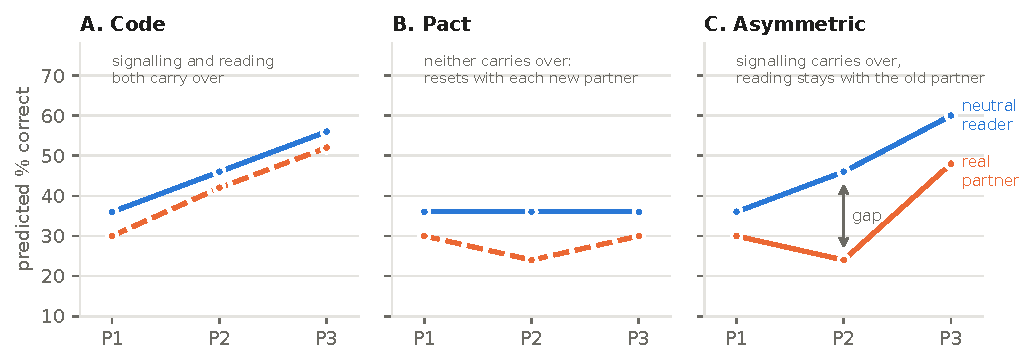
\includegraphics[width=\linewidth]{figH_hypotheses}
\figurenote{Schematic predictions, not data. Blue: proportion of a Sender's signals read correctly by a neutral reader with no history with that Sender (signalling). Orange: success with the real partner (signalling and reading together). P1--P3 are the three partner phases.}
\end{figure}

The hypothesis distinguishes two things players learn with each partner: how to signal and how to read signals. \emph{If} what players learn about signalling carries over directly to a new partner, but they must learn anew how to read that partner's signals, \emph{then} signals should become clearer across partner changes even as success drops just after each change. This distinction yields four predictions and an exploratory prediction, each with a null alternative:
\begin{enumerate}
\item[H1a.] Signals become easier for a neutral reader to interpret across phases, even as partners change (H0: legibility does not change across phases).
\item[H1b.] In the phase after a partner switch, real Receivers succeed less often than a neutral reader does when interpreting the same signals (H0: real and neutral success do not differ).
\item[H1c.] When early and late signals are each paired with early and late Receivers, later signals contribute more to success than later Receivers do (H0: Sender and Receiver effects are equal).
\item[H1d.] Each player's signalling style shifts toward that of their current partner, but not toward that of the group as a whole (H0: no greater shift toward the current partner than toward a non-partner).
\item[H1e.] (Exploratory.) As a group, players converge on signal forms that anyone can read rather than on forms specific to their own tournament (H0: the mix of forms does not shift toward legible forms, or shifts toward tournament-specific forms).
\end{enumerate}
The code and pact accounts each predict one part of this pattern: the code account predicts H1a but not H1b, and the pact account predicts H1b but not H1a. Only the asymmetric account predicts both.

% ======================================================================
\section{Method}

\subsection{Participants}

Sixteen Dartmouth College students took part, all recruited in and around the college library as a convenience sample. They played in three tournaments with six, six, and four players, respectively.
% TODO(author): add age range, gender, how consent was obtained, and whether participants were compensated.
Participation was voluntary. Players joined using a first name or nickname, and no identifying information was stored with the game logs.

\subsection{Design}

The study used a within-subjects design in which \emph{partner phase} was the independent variable (phase 1, first partner; phase 2, new partner; phase 3, new or reunited partner). The dependent variables were (a) communicative success on each round, defined as the Receiver placing the token on the correct tile in the correct orientation; (b) the legibility of each Sender signal, measured by whether a neutral reader read the signal correctly; and (c) the position of each Sender signal in a style space (described below). The board, time limit, goal set (each goal was used equally often), and feedback given to players were held constant across phases.

The partner schedule was not fully balanced. In phase 2, all pairs were new except for one pair in tournament 2. In phase 3, all three pairs in tournament 1 and one pair in tournament 2 were \emph{reunited} with their phase-1 partners, whereas tournament 3 used new partners throughout. Where relevant, we therefore report phase-3 rounds separately for new and reunited partners.

\subsection{Materials and Apparatus}

We reimplemented the TCG \parencite{deruiter2010} as a web application (Node.js server, browser client) based on the course's \enquote{Crack the Vault} version. Players could join from their own devices, and the experimenter controlled pairing through an administrator dashboard. In each round, one player took the role of Sender and saw the goal: one of nine tiles for the Receiver's triangle and one of eight directions for it to point. The Sender used the arrow keys to move a circle for up to nine seconds (20 seconds on each player's first turn in each role) while the Receiver watched. The Receiver then placed and rotated the triangle. The only feedback either player saw was SUCCESS or FAIL. Roles alternated every round. Every key press and its timing were logged.

\begin{figure}[t]
\caption{The Task and the Tournament Design}
\label{fig:game}
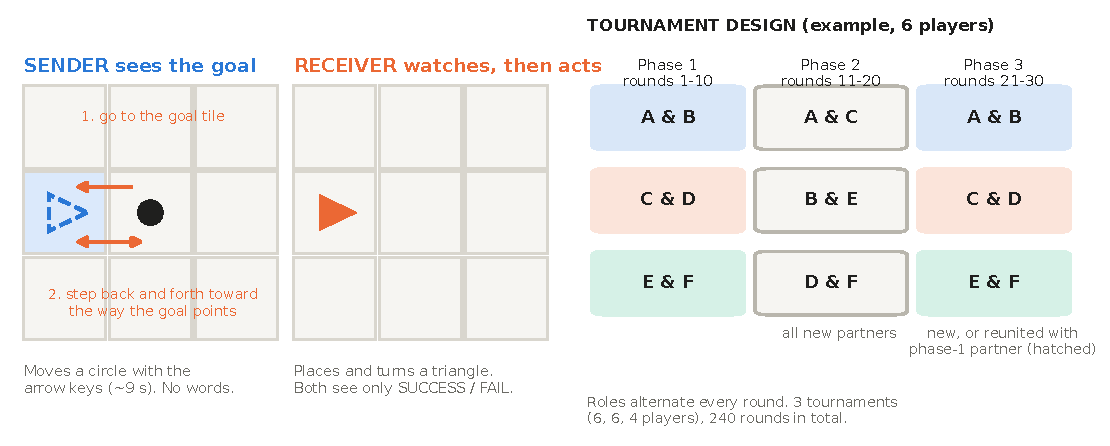
\includegraphics[width=\linewidth]{fig1_game}
\figurenote{Left: one round. The goal (dashed triangle) is the middle-left tile, pointing right; the Sender goes to the goal tile and then steps back and forth toward the way the goal points, and the Receiver places and turns its own triangle. Right: the re-pairing schedule for an example six-player tournament. Hatched pairs in phase 3 are reunions, which occurred in tournament 1 and for one pair in tournament 2.}
\end{figure}

\subsection{Procedure}

Players opened the game on their devices, entered a name, and waited in a lobby. Once all players had joined, the experimenter started the tournament. Each tournament consisted of three phases of ten rounds. Between phases, all players saw a message telling them they would play with a different partner, and the server assigned new partners according to the schedule (Figure~\ref{fig:game}). The 30 rounds of a tournament took 10 to 11 minutes of play (10.6, 11.3, and 10.0 minutes from the start of the tournament to the last round), or about 21 seconds per round including feedback and the transition to the next round. Of this, active play averaged 15.4 seconds per round ($SD = 5.3$): 8.9 seconds for the Sender's turn and 6.5 seconds for the Receiver's. The three tournaments yielded 240 rounds in total, 80 in each phase.

\subsection{Analysis}

\subsubsection{Preprocessing}

The key presses in each Sender turn were summarized as a series of readable steps (for example, \enquote{went to top; wiggled top$\leftrightarrow$center $\times 5$; long pause on top; time ran out}). The summaries preserved the final tile in 100\% of turns and the hand-coded strategy in 93\%. Because the summaries omitted intermediate tiles and pauses shorter than one second, the exact arrow-key sequence could be recovered in only 59\% of turns. No rounds were excluded.

\subsubsection{Measuring Legibility: A Neutral Reader}

To measure how readable a signal was without relying on familiarity with a particular partner, we used a large language model (GPT-6.1 Terra) as a simulated Receiver. We gave the model the rules and five complete games from \emph{other} tournaments, then asked it where to place the triangle after reading each Sender turn. Because the model had no history with any player, we used its accuracy as a measure of how legible each signal was to an outsider. The model read all 240 real Sender turns. For each turn $t$, we recorded a binary legibility score $\ell_t \in \{0, 1\}$ alongside the real outcome $y_t \in \{0, 1\}$.

\subsubsection{Separating Signalling From Reading: A Counterfactual Design}

To separate the contributions of Senders and Receivers, we used a $2 \times 2$ counterfactual design. Within each tournament, we gave a simulated Receiver each real player's history up to either the end of phase 1 (\emph{early Receiver}) or the start of phase 3 (\emph{late Receiver}). Each version decoded eight phase-1 signals and eight phase-3 signals from \emph{other} players, excluding any signals the player had actually received, for 512 decodes in all. The Sender effect measured the gain from later signals while holding the Receiver fixed. The Receiver effect measured the gain from more history while holding the signals fixed. Their interaction tested whether late signals worked especially well for late Receivers, as a shared convention would predict. We obtained confidence intervals by resampling Receivers (3,000 bootstrap samples).

\subsubsection{Measuring Style: An Embedding Built From Similarity Judgments}

We mapped signalling style from similarity judgments rather than hand-coded strategy labels, following the odd-one-out approach used to map human object concepts \parencite{hebart2020}. For each triplet, a language-model judge saw three Sender turns, each with its own goal, and selected the turn whose signalling strategy differed most from the other two. We collected 2,649 such triplets across all 240 turns, along with 1,560 two-choice probes (4,209 judgments). We then fitted a three-dimensional embedding by maximum likelihood, placing turns judged similar close together. Each turn $i$ was assigned a position $\mathbf{x}_i \in \mathbb{R}^3$. Selecting $k$ as the odd one out of $\{i, j, k\}$ identifies $i$ and $j$ as the most similar pair. The model assigns this choice the probability
\begin{equation}
P(k \text{ odd} \mid \mathbf{x}) = \frac{\exp(-\lVert \mathbf{x}_i - \mathbf{x}_j \rVert^2)}{\exp(-\lVert \mathbf{x}_i - \mathbf{x}_j \rVert^2) + \exp(-\lVert \mathbf{x}_i - \mathbf{x}_k \rVert^2) + \exp(-\lVert \mathbf{x}_j - \mathbf{x}_k \rVert^2)}.
\end{equation}
The fitted positions maximize the sum of the log probabilities across all judgments. The embedding with three dimensions best predicted held-out judgments. For analyses of change, we subtracted the mean position of turns with the same goal from each turn's position,
\begin{equation}
\mathbf{r}_t = \mathbf{x}_t - \frac{1}{|G_t|}\sum_{u \in G_t} \mathbf{x}_u,
\end{equation}
where $G_t$ is the set of turns with the same goal as turn $t$ (each goal occurred eight times). Distances were then computed relative to these goal means to reflect differences in style rather than goal.

The embedding showed acceptable internal validity. The judge gave the same answer on 84\% of reshuffled triplets, which served as a ceiling. The embedding predicted 70\% of held-out triplets (chance 33\%) and 81\% of held-out pairwise probes (chance 50\%). Placing a new turn in the embedding using ten judgments allowed it to predict 72\% of the other judgments for that turn. The three axes were interpretable: signalling a direction versus simply going to the goal, stepping toward versus away from the goal direction, and marking the center versus wiggling at the goal. Because the original prompt listed example strategies, we removed the examples and repeated the procedure.

\subsubsection{Inferential Tests}

Changes in success and legibility across phases were assessed using logistic regression with phase as a predictor and $\chi^2$ tests. McNemar's test compared the neutral reader and the real Receiver on the same signals, and Fisher's exact test compared proportions between groups. Because each Sender contributed several turns, the main effects were rechecked using logistic generalized estimating equations with an exchangeable correlation structure and clustering by Sender. A reader-by-phase interaction tested whether the gap between the neutral reader and the real partner was larger after the first switch than in phase 1. To test for the influence of a partner's style, each player's next turn was regressed on their own previous turn and their current partner's latest turn, $\mathbf{r}_{p,\,t+1} = a_1\,\mathbf{r}_{p,\,t} + a_2\,\mathbf{r}_{q(p),\,t} + \boldsymbol{\varepsilon}$. The analysis pooled the three dimensions and used standard errors clustered by player ($n = 224$ turns with a preceding turn). An extended model added the mean of the player's own past successful turns, and a placebo model replaced the partner with a random non-partner from the same tournament. To test for group-specific signal forms, each Sender turn was assigned a form label using rules (for example, a wiggle toward the goal, a sideways wiggle, or direct movement to the goal). The probability that two turns in the same tournament and phase shared a form was compared with the probability obtained by shuffling tournament labels within phase (1,000 permutations).

\subsubsection{A Generative Model}

To test whether the partner pull could account for the group-level pattern, we fitted a generative model. In the model, each player's next turn was a weighted combination of their own last turn, their partner's last turn, and their own past successful turns. Success depended on how legible the signal was and how closely it matched what the Receiver had come to expect. We then ran the model 300 times using each tournament's actual partner schedule. For a separate comparison, we tested whether large language models could predict a player's next move given that player's history. We also had the language models play whole tournaments in closed loop.

% ======================================================================
\section{Results}

Three findings emerged. Senders' signals became easier for anyone to read, while understanding between new partners improved more slowly. Signal clarity set an upper limit on understanding, but within that limit, the ability to read a new partner's signals appeared to recover. Finally, groups converged on the most readable signal form through mutual influence between partners rather than through group-specific conventions.

\subsection{Signals Became Clearer, and New Partners Lagged Behind (H1a, H1b)}

Real success was 29\% in phase 1 (23 of 80 rounds), 24\% in phase 2 (19 of 80), and 49\% in phase 3 (39 of 80), $\chi^2(2) = 12.52$, $p = .002$. The decline from phase 1 to phase 2 was not statistically significant (Fisher's exact $p = .59$), whereas the increase from phase 2 to phase 3 was ($p = .002$). By contrast, the neutral reader's accuracy in decoding Senders' signals rose steadily across phases: 36\%, 46\%, and 61\% (29, 37, and 49 of 80), OR $= 1.67$ per phase, $p = .002$ (Figure~\ref{fig:gap}). This pattern supports H1a: signals became more legible even as partners changed.

\begin{figure}[t]
\caption{Legibility Rose Steadily While Real Success Dipped After the First Switch}
\label{fig:gap}
\centering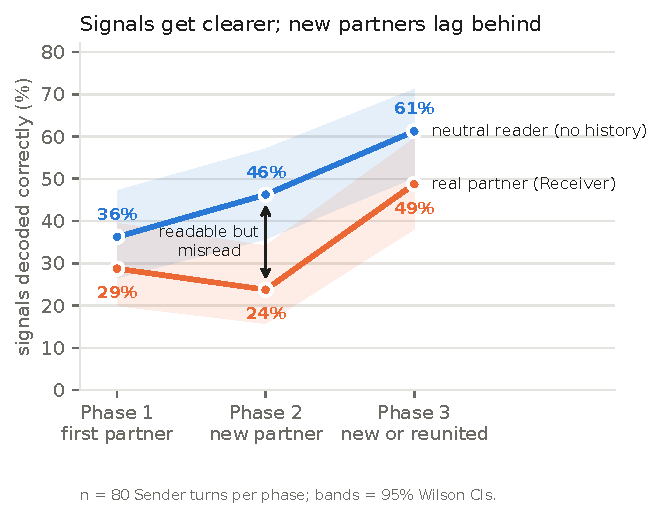
\includegraphics[width=0.78\linewidth]{figG_gap}
\figurenote{The same signals, read by a neutral reader with no history (blue) and by the players' real partners (orange). Bands are 95\% Wilson confidence intervals; $n = 80$ Sender turns per phase.}
\end{figure}

In phase 2, the gap between the two was large. On the same 80 signals, the neutral reader succeeded on 37 and the new partner on 19; in 27 rounds the neutral reader was right and the partner wrong, and in only 9 the reverse, McNemar $p = .004$. There was no reliable gap in phase 1 ($p = .34$) and a smaller one in phase 3 ($p = .052$). The gap was larger in phase 2 than in phase 1 (reader-by-phase interaction: OR $= 1.96$, $p = .044$), so the neutral reader was not simply better than people across the board, and the main effects held when repeated turns by the same Sender were taken into account (legibility OR $= 1.67$, $p = .004$; phase-2 gap OR $= 2.76$, $p = .005$). The gap appeared in tournaments 1 and 2 and was small in tournament 3 (30\% vs.\ 25\%). It also did not open at once: in the first five rounds with a new partner, real Receivers and the neutral reader did about equally well (31\% vs.\ 34\%); in the last five, the neutral reader rose to 57\% while real Receivers fell to 17\%. This supports H1b: after a switch, Senders were producing clearer signals than before, but their new partners read them differently.

\subsection{The Signal Set a Ceiling, and Reading Recovered Within It (H1c; Exploratory)}

Partners' understanding was limited by the clarity of the signal. To examine this, we grouped rounds by whether the neutral reader had interpreted the signal correctly (Table~\ref{tab:ceiling}); this analysis was unplanned and is exploratory. When the neutral reader had not interpreted the signal correctly, real partners succeeded 21\% of the time (26 of 125). This rate varied little across phases (22\%, 21\%, 19\%), even though by phase 3 many pairs had played together before. When the neutral reader had interpreted the signal correctly, real partners succeeded 48\% of the time (55 of 115), Fisher's exact $p < .001$. Partners found the correct tile equally often in both cases (83\%); the difference was in how often they got the direction right (25\% correct vs.\ 53\%). These results suggest that familiarity with the Sender seldom compensated for a signal the neutral reader could not interpret. In that sense, the signal sets a ceiling on what any reader can recover.

\begin{table}[t]
\caption{Real Partners' Success by Whether a Neutral Reader Could Read the Signal}
\label{tab:ceiling}
\begin{tabular}{lccc}
\toprule
Signal & Phase 1 & Phase 2 & Phase 3 \\
\midrule
Readable to the neutral reader & 41\% (12/29) & 27\% (10/37) & 67\% (33/49) \\
Unreadable to the neutral reader & 22\% (11/51) & 21\% (9/43) & 19\% (6/31) \\
\bottomrule
\end{tabular}
\end{table}

Within that ceiling, reading appeared to recover. For readable signals, success among actual Receivers went from 41\% to 27\% to 67\% across phases. The clearest comparison is between Receivers who met a new partner in phase 2 and those who did so in phase 3, because the neutral reader found the two sets of signals about equally clear (46\% of 70 vs.\ 48\% of 40). Actual Receivers nevertheless did better in the later phase, 40\% versus 24\% (16 of 40 vs.\ 17 of 70), Fisher's exact $p = .09$. For signals the neutral reader could read, they succeeded on 53\% (10 of 19) versus 25\% (8 of 32). This pattern is consistent with people getting better at reading a new partner, though the difference was not statistically reliable and the new pairs in phase 3 came only from tournaments 2 and 3. Individual success rates also varied more among Receivers than among Senders: they ranged from 7\% to 67\% as a Receiver and from 20\% to 53\% as a Sender.

The size of the reading effect remains uncertain. The planned counterfactual test used simulated Receivers. The same Receivers decoded later signals more accurately than earlier ones by 14 percentage points, 95\% CI [5, 22], whereas giving a Receiver more history improved decoding by 5 points [$-4$, 14], with no interaction ($-1$ point [$-12$, 11]). The Sender effect was reliable and the Receiver effect was not, but the two effects did not differ reliably (difference 9 points [$-7$, 24]). Thus, H1c is supported in direction only. The reading effect was positive in both the simulated and the real comparison, but neither established it. The reunion results also warrant caution. In phase 3, reunited pairs succeeded more often than new pairs (57\% vs.\ 40\%, 23 vs.\ 16 of 40; Fisher's exact $p = .18$), but their Senders' signals were also more legible to the neutral reader (75\% vs.\ 48\%, $p = .021$). Reunions were concentrated in tournament 1, so the effect of resuming a pact cannot be separated from that of having better Senders.

\subsection{Groups Converged on the Most Readable Form, Not on Dialects (H1e)}

If each tournament were developing its own small language, turns within a tournament should share forms more often than turns from different tournaments. They did not. The probability that two turns in the same tournament and phase used the same form was no higher than when tournament labels were shuffled (0.20 vs.\ 0.20, permutation $p = .31$). Instead, the tournaments changed in the same direction (Figure~\ref{fig:lex}). The share of turns that signalled any direction rose from 69\% in phase 1 to 88\% in phase 2, and the \emph{pointer} form, a wiggle from the goal in the direction it points, rose from 15\% to 36\% of turns (Fisher's exact $p = .003$), led by tournaments 1 and 2. This was the most legible form in the game: the neutral reader decoded pointer turns correctly 71\% of the time, compared with 39\% for all other forms ($p < .001$), and actual partners decoded pointer turns correctly 57\% of the time. The style map showed a similar pattern at a broader level: its one robust distinction was between turns that attempted to signal a direction and turns that simply went to the goal. The shift did not yield a fixed convention: in phase 3 the pointer share fell back to 21\% as some players returned to simply marking the goal. Because the tournaments never met, this convergence cannot reflect copying between groups. The pattern is consistent with pairs independently adopting the form that was easiest to read. The results thus supported H1e for the direction of change, but not for the emergence of a stable group convention.

\begin{figure}[t]
\caption{Signal Forms by Tournament and Phase}
\label{fig:lex}
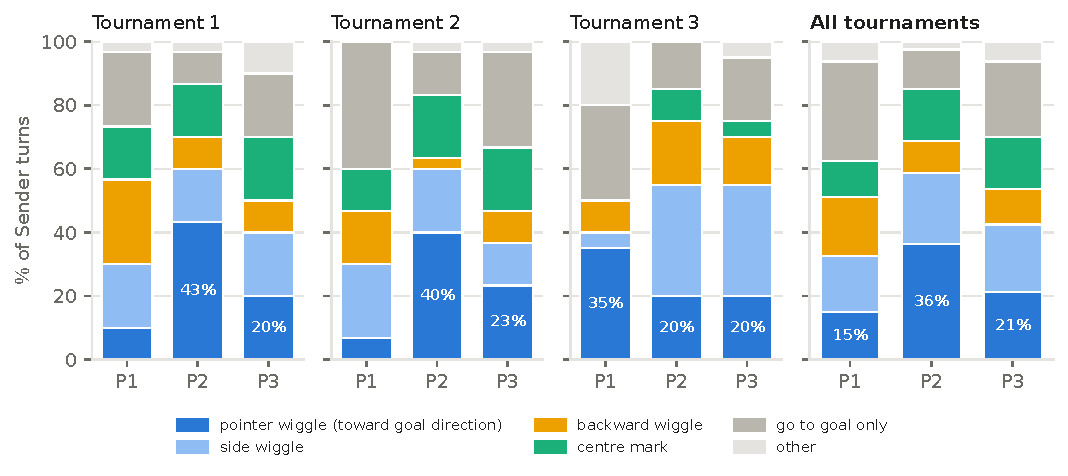
\includegraphics[width=\linewidth]{figL_lexicon}
\figurenote{Rule-based form label of every Sender turn. The pointer wiggle (dark blue) was the most legible form for the neutral reader (71\% correct vs.\ 39\% for other forms).}
\end{figure}

\subsection{The Pull Came From the Current Partner (H1d)}

Convergence occurred pair by pair. In the style space, partners' turns were always closer to each other than to non-partners' turns (Figure~\ref{fig:conv}). Regressing each player's next turn on their own previous turn and their current partner's latest turn yielded weights of 0.25 ($p < .001$) and 0.13 ($p = .002$), respectively, whereas substituting a random non-partner yielded a weight of $-0.08$ ($p = .004$). The pull toward the partner was evident in phase 1 (0.16, $p = .014$) and phase 3 (0.17, $p = .041$), but not in phase 2 (0.01), and was replicated using a judge who saw no example strategies (0.14, $p = .009$). The effect was modest: the player's own turn and the partner's turn together explained 9.4\% of the variance in the player's next turn. There was no evidence of a group-wide style. A judge could not identify which tournament a turn came from at above-chance levels (50\%, chance 50\%), and styles did not become more fixed as partners played more games together (slope $+0.001$ per game, $p = .96$). The results therefore supported the pairwise form of H1d: styles shifted toward the current partner, not toward the group.

\begin{figure}[t]
\caption{Convergence in Signalling Style}
\label{fig:conv}
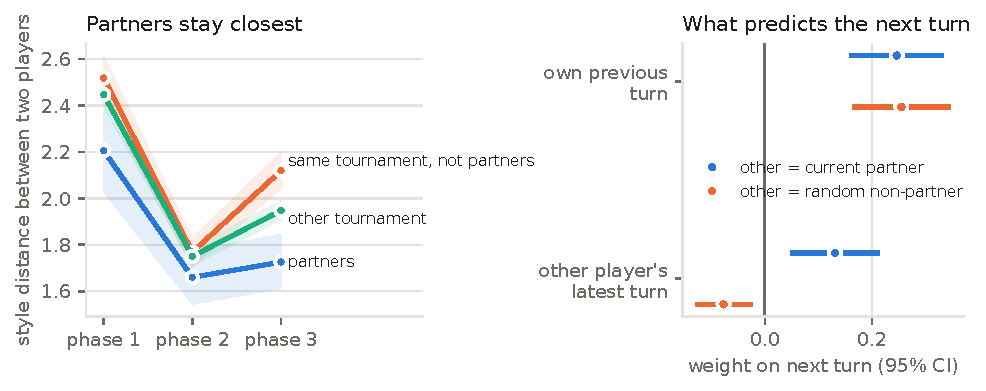
\includegraphics[width=\linewidth]{fig5_convergence}
\figurenote{Left: style distance between two players' turns in the same phase. Right: weights on a player's next turn, with 95\% confidence intervals clustered by player.}
\end{figure}

\subsection{What the Models Did Not Reproduce}

Two modelling exercises marked the limits of this account. A generative model built from the fitted pulls, simulated 300 times on the real partner schedules, reproduced the partner alignment but not the success curve: simulated success was 31\%, 38\%, and 34\% in phases 1--3 against the real 29\%, 24\%, and 49\%, apparently because the three-dimensional style map does not capture what makes a signal readable (legibility estimated through it was flat, about 47\% in every phase). Language models given a player's real history predicted the Sender's strategy 57\% of the time and the Receiver's interpretation 63\% of the time (GPT-6.1 Terra; history-free baseline 43\% and 49\%), but they predicted less change than people make, and when they played entire tournaments they succeeded 48\%, 68\%, and 60\% of the time with no cost of switching partners. Simulated players coordinated far more easily than people did.

% ======================================================================
\section{Discussion}

How does shared understanding spread through a group, and how much of what a pair has worked out can either person take to a new partner? If it works like a code, everything the pair has learned should carry over. If it works like a pact, understanding should have to be built anew with each partner. Neither account fits the data on its own. As the code account predicts, signals became steadily easier for a reader who had never met the Sender to interpret. Yet after a switch, actual partners misread these clearer signals, as the pact account predicts. In the counterfactual decomposition, later signals reliably improved reading, whereas Receiver experience did not; statistically, however, the two effects could not be distinguished. We therefore reject the null hypotheses for H1a and H1b, for the pairwise form of H1d, and, with respect to the direction of change, for H1e. H1c was supported in direction only. The evidence favors a version of the asymmetric account: clearer signals benefit new partners directly, whereas reading must be relearned with each partner. This does not mean that reading fails to improve. Rather, the exploratory analyses suggest that signals limit how much can be understood and that, within this limit, Receivers became better at reading new partners.

\subsection{How Shared Signals Develop in a Group}

These results suggest how conceptual pacts \parencite{brennan1996,garrod1987} might become community conventions \parencite{garrod1994,fay2010}. Each pair works out its own agreement, but not all of that agreement travels equally well. As Senders make their signals more explicit, those signals become easier for outsiders to read. Receivers, by contrast, learn how one particular Sender uses signals and must learn anew with each partner, perhaps more quickly each time. As players rotate, signals that a new partner can read are more likely to persist. This pattern echoes the finding that outsiders interpret signs refined in a community more easily than signs refined by an isolated pair \parencite{fay2008}. It also fits the conceptual alignment framework \parencite{stolk2016,stolk2020}: if Receivers interpret signals in light of what they have learned about a particular partner, a decline after a switch is to be expected. The group-level results fit this account. No tournament developed a dialect of its own; pairs in every tournament moved toward the same pointer form, the one outsiders could read most easily. A community can thus come to share a vocabulary without ever agreeing on it as a group. Forms that make sense to new partners persist, while those that depend on a particular pair fall away. The account also yields a prediction: newcomers should be understood before they understand others.

\subsection{Limitations}

Several limits qualify these conclusions. The convenience sample was small (16 players, 240 rounds), and several effects, including the dip itself, were statistically uncertain. In the phase-3 reunions, partner familiarity and tournament were confounded: what looks like the renewal of a pact may instead reflect better signallers. The \enquote{neutral} reader had already learned the task from five complete games from other tournaments. Some of the rise in legibility may therefore reflect a growing resemblance to the signals those groups used later. The model may also favor readily understood forms such as the pointer. The counterfactual Receivers were simulated, and language models adapted less than people did. That comparison did not establish that Senders contributed more than Receivers, so it remains unclear how much people improved at reading signals. The exploratory comparisons suggest that they did improve. The style map, too, depends on a language model's judgments. Several tests were conducted without correction for multiple comparisons, the key gap-by-phase interaction was only just significant ($p = .044$), and the ceiling and group-level analyses were exploratory. Finally, it remains an open question how much a wordless, nine-second laboratory game can tell us about conversation.

\subsection{Future Directions}

Two steps would help clarify what players learn about one another. First, further tournaments could use a balanced schedule in which no pair plays together again and every player meets several new partners. This would remove the main confound and test whether a shared convention emerges over time. Second, people, rather than a language model, could interpret signals from players they have never met, both early and late in their own session. Comparing their performance would measure directly how much their ability to read unfamiliar players improves.

\subsection{Conclusion}

When strangers devise a way to communicate without words, they learn two things that carry over differently. Senders learn to make their meaning clear in a form that new partners can understand. Receivers, by contrast, learn to interpret the signals of a particular partner. With each new partner, they must learn to do this again, although the task may become easier with practice. Even an experienced Receiver cannot recover what the signal does not convey. This distinction helps explain how an agreement between two people might become a convention for a group: as pairs settle on forms that others can readily interpret, the clearest signals may spread, much as words might take hold in an emerging language.

\printbibliography

\appendix
\section{Supplemental Materials: Analysis Code}

The code for the online game, all analysis scripts, and the source files for this report are publicly available at \url{https://github.com/dylan518/tcg-ladder}. The game logs are kept out of the public repository to protect participants' privacy, but readers may request them from the author. The main scripts are listed below by purpose:
\begin{itemize}
\item \texttt{engine.js}, \texttt{tournament.js}, \texttt{public/}: run the online game, pair players for the tournament, and log play.
\item \texttt{analysis/tokenize\_games.py}, \texttt{analysis/models/readable.py}: turn key presses into readable steps.
\item \texttt{analysis/models/cf\_encode\_decode.py}: assess legibility for a neutral reader and perform the $2 \times 2$ counterfactual decoding.
\item \texttt{analysis/models/strategy\_embed.py}, \texttt{analysis/models/eval\_embeddings.py}: handle triplet judgments and the style embedding.
\item \texttt{analysis/models/reading\_ceiling.py}: explore the signal ceiling and reading with new partners.
\item \texttt{analysis/models/convergence.py}: analyze distances and run the style-update regressions.
\item \texttt{analysis/label\_strategies.py}: label signal forms by hand for analysis at the group level.
\item \texttt{analysis/models/group\_model.py}: implement the generative model and run its simulations.
\item \texttt{analysis/models/fullgame\_sonnet.py}, \texttt{analysis/models/llm\_validity.py}: use language models to model players.
\item \texttt{paper/make\_figures.py}, \texttt{paper/make\_figures\_v2.py}: produce all figures.
\end{itemize}

\end{document}
